\documentclass{beamer}
\usepackage[british,spanish]{babel}
\usepackage[utf8]{inputenc}

\usepackage{hyperref}
%\hypersetup{colorlinks=false,linkbordercolor=red,linkcolor=green,pdfborderstyle={/S/U/W 1}}

\usepackage{multirow}

\usepackage{textcomp}

\usepackage{listings}
\lstloadlanguages{Ruby}
\usepackage{cancel}
\usepackage{adjustbox}
\usepackage{lstcustom}

\usepackage{amsmath}

\usepackage{color}
\definecolor{light-gray}{gray}{0.80}
\definecolor{lstbackgroundshellcolor}{named}{light-gray}

\usepackage{tikz}
\newcommand*\circled[1]{\tikz[baseline=(char.base)]{
            \node[shape=circle,draw,inner sep=2pt] (char) {#1};}}

\usepackage[normalem]{ulem}

%\usepackage[acronym,xindy,toc]{glossaries}

\usepackage[acronym,xindy,toc]{glossaries}
\makeglossaries
%\usepackage[xindy]{imakeidx}
%\makeindex


\newcommand{\comment}[2]{#2}

\newcommand{\commandinline}[1]{\lstinline[basicstyle=\small\lstfontfamily]{#1}}
\newcommand{\outputcommand}[1]{\color{darkgreen}{#1}}

\graphicspath{ {./images/} }

\title{Building a Scalable Architecture with Amazon SQS}
%\subtitle[short subtitle]{long subtitle}
\author[C. Cuenca, F. Quintana]{Carmelo Cuenca-Hernández and Francisca Quintana-Domínguez}
%\institute{Escuela Universitaria de Informática}
%\date[04/2013]{Abril - 2013}
\date{}
\titlegraphic{
\includegraphics[width=0.5 \textwidth]{./images/logo_ulpgc_version_horizontal_rgb.eps}}


\pgfdeclareimage[widiamth=2.0\baselineskip]{ulpgc-logo}{images/logosimbolo_secundario_version_vertical}
\setbeamertemplate{footline}{\raisebox{-2ex}{\pgfuseimage{ulpgc-logo}}
  \usebeamerfont{date in head/foot}\insertshortdate{}\hfill
  \usebeamertemplate{navigation symbols}\hfill
  \insertframenumber{}/\inserttotalframenumber}
\setbeamertemplate{sidebar right}{}


\usetheme{Antibes}
%\usetheme{Berlin}

%\usetheme{Warsaw}
%\usecolortheme{albatross}

\selectlanguage{british}



\begin{document}

%
\includegraphics[width= 1.0 \textwidth]{logos3.eps}
\begin{frame}
	\titlepage
\end{frame}


\section*{Outline}
\begin{frame}[fragile, allowframebreaks]
  \frametitle{Outline}
  %\tableofcontents%[part=1,pausesections]
  %\tableofcontents[currentsection,currentsubsection, sectionstyle=show] 
  \tableofcontents[currentsection,sectionstyle=show,hideothersubsections]
\end{frame}

%%%%%%%%%%%%%%%%%%%%%%%%%%%%%%%%%%%%%%%%%%%%%%%%%%%%%%%%%%%%%%%%%%%%%%%%%%%%%%
%\newacronym{<label>}{<abbrv>}{<full>}
%\glsreset{<label>}
%\glsresetallQueue-Centric Workflow Pattern
%\acrlong{<label>}
%\acrfull{<label>}Elastic Load Balancing
%\acrshort{<label>}
%\input{../glossary}

\newacronym{acl}{ACL}{Access Control List}
\newacronym{api}{API}{Application Programming Interface}
\newacronym{aws}{AWS}{Amazon Web Services}
\newacronym{cli}{CLI}{Command Line Interface}
\newacronym{css}{CSS}{cascading style sheets}
\newacronym{ebs}{EBS}{Elastic Block StoAWS Identity an Access Managementrage}
\newacronym{ec2}{EC2}{Amazon Elastic Compute Cloud}
\newacronym{elb}{ELB}{Elastic Load Balancing}
\newacronym{iam}{IAM}{Identity Access Management}
\newacronym{ror}{RoR}{{\href{http://rubyonrails.org/}{Ruby on Rails}}}
\newacronym{rds}{RDS}{Relational Database Service}
\newacronym{rvm}{RVM}{{\href{https://rvm.io/}{Ruby Version Manager}}}
\newacronym{s3}{S3}{Simple Storage Service}
\newacronym{sqs}{SQS}{Amazon Simple Queue Service}
%%%%%%%%%%%%%%%%%%%%%%%%%%%%%%%%%%%%%%%%%%%%%%%%%%%%%%%%%%%%%%%%%%%%%%%%%%%%%%
\end{document}

\section{Amazon Simple Queue Service}
\begin{frame}[fragile]
\frametitle{Amazon Simple Queue Service}
\begin{itemize}
\item \acrfull{sqs} is a fast, reliable, scalable, fully managed message queuing service. SQS makes it simple and cost-effective to decouple the components of a cloud application. You can use SQS to transmit any volume of data, at any level of throughput, without losing messages or requiring other services to be always available

\item With \acrshort{sqs}, you can offload the administrative burden of operating and scaling a highly available messaging cluster, while paying a low price for only what you use.

\item Service Highlights
\begin{itemize}
\item Reliable. Amazon \acrshort{sqs} runs within Amazon’s high-availability data centers, so queues will be available whenever applications need them. To prevent messages from being lost or becoming unavailable, all messages are stored redundantly across multiple servers and data centers
\item Scalable
\item Secure
\item Inexpensive
\end{itemize}

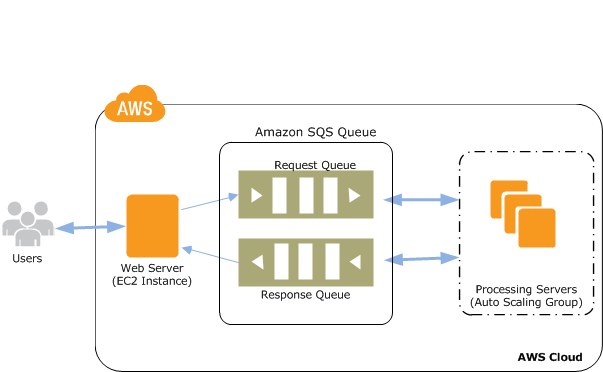
\includegraphics[width=1.0 \textwidth]{sqs-as-workflow.png}
\end{itemize}
\end{frame}
%%%%%%%%%%%%%%%%%%%%%%%%%%%%%%%%%%%%%%%%%%%%%%%%%%%%%%%%%%%%%%%%%%%%%%%%%%%%%





\begin{frame}[fragile,allowframebreaks]
\frametitle{Queue-Centric Workflow Pattern}
\begin{itemize}
\item The Queue-Centric Workflow Pattern is used in web aplications to decouple comu
nication between the web tier (which implements the user interface) and the service tier
(where business processing happens)
\end{itemize}
\end{frame}



%%%%%%%%%%%%%%%%%%%%%%%%%%%%%%%%%%%%%%%%%%%%%%%%%%%%%%%%%%%%%%%%%%%%%%%%%%%%%%
\section{Homework}
%%%%%%%%%%%%%%%%%%%%%%%%%%%%%%%%%%%%%%%%%%%%%%%%%%%%%%%%%%%%%%%%%%%%%%%%%%%%%
\begin{frame}[fragile]
\frametitle{Homework}
\begin{itemize}
\item ???
\end{itemize}
\end{frame}

%%%%%%%%%%%%%%%%%%%%%%%%%%%%%%%%%%%%%%%%%%%%%%%%%%%%%%%%%%%%%%%%%%%%%%%%%%%%%%

%%%%%%%%%%%%%%%%%%%%%%%%%%%%%%%%%%%%%%%%%%%%%%%%%%%%%%%%%%%%%%%%%%%%%%%%%%%%%%

